
%Copyright (C) 2016 by Krishneel@JSK Lab, The University of Tokyo

%Copyright (C) 2016 by Krishneel@JSK Lab, The University of Tokyo

\documentclass{standalone}
\usepackage{footnote}
\usepackage{hyperref}
\usepackage{graphicx}
\usepackage{fancyhdr}

\renewcommand\footnoterule{%
  \kern-3\p@
  \hrule\@width2.5cm
  \kern2.6\p@
}
\makeatother

\begin{document}

\subsection{Platforms}
We customized the developer platform of DJI M100 as shown in Fig.\ref{figure:task1-platform}(Top). We used two Nvidia Jeston TX1 to distribute the load especially caused image processing. Those two processors are connected via a wired internal network.
We also apply the camera with fisheye lens which has $250^\circ$ to have a wide view for tracking, as well as the optical-flow $\&$ sonar sensor units to estiamte the ego-motion of the UAV. The system framework can be described as Fig.\ref{figure:task1-platform}(Down), which the processing nodes inside the porcessers will be explained later.

\begin{figure}[h]
    \begin{center}
        \begin{minipage}{\hsize}
          \begin{center}
      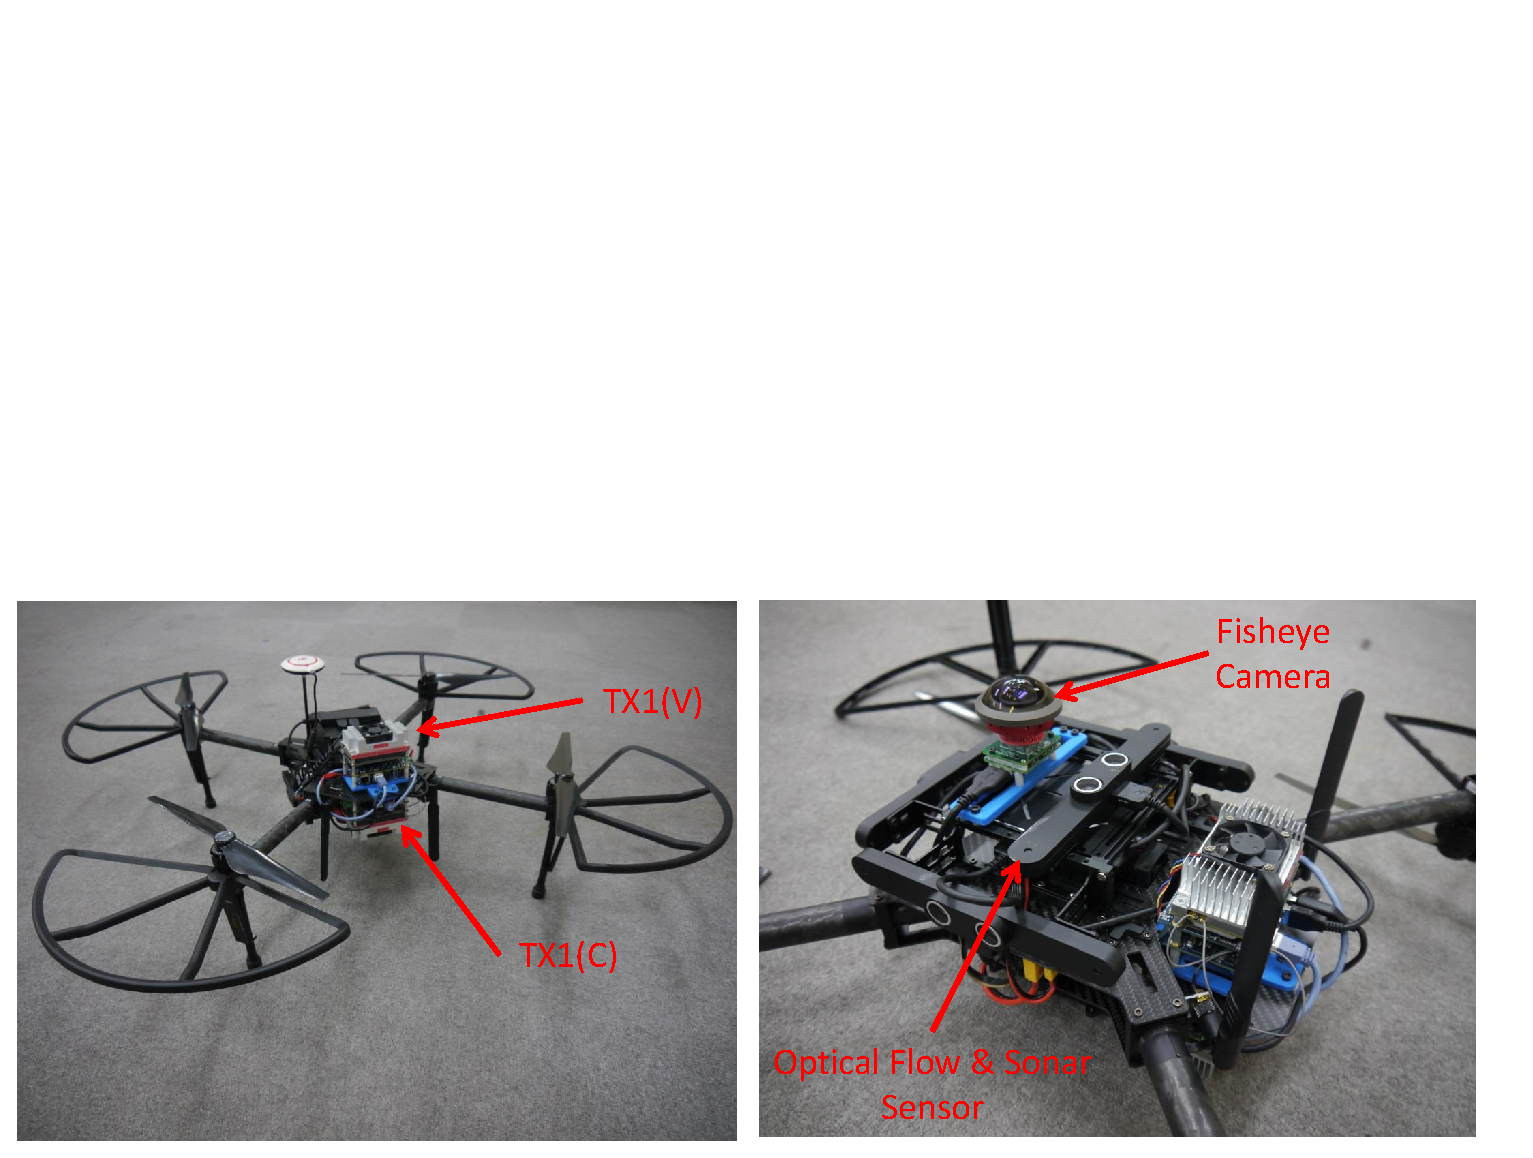
\includegraphics[clip, bb= 0 0 700 260, width=\columnwidth]{sections/task1/images/task1_hardware.eps}
          \end{center}
        \end{minipage}
        \begin{minipage}{1.0\hsize}
          \begin{center}
      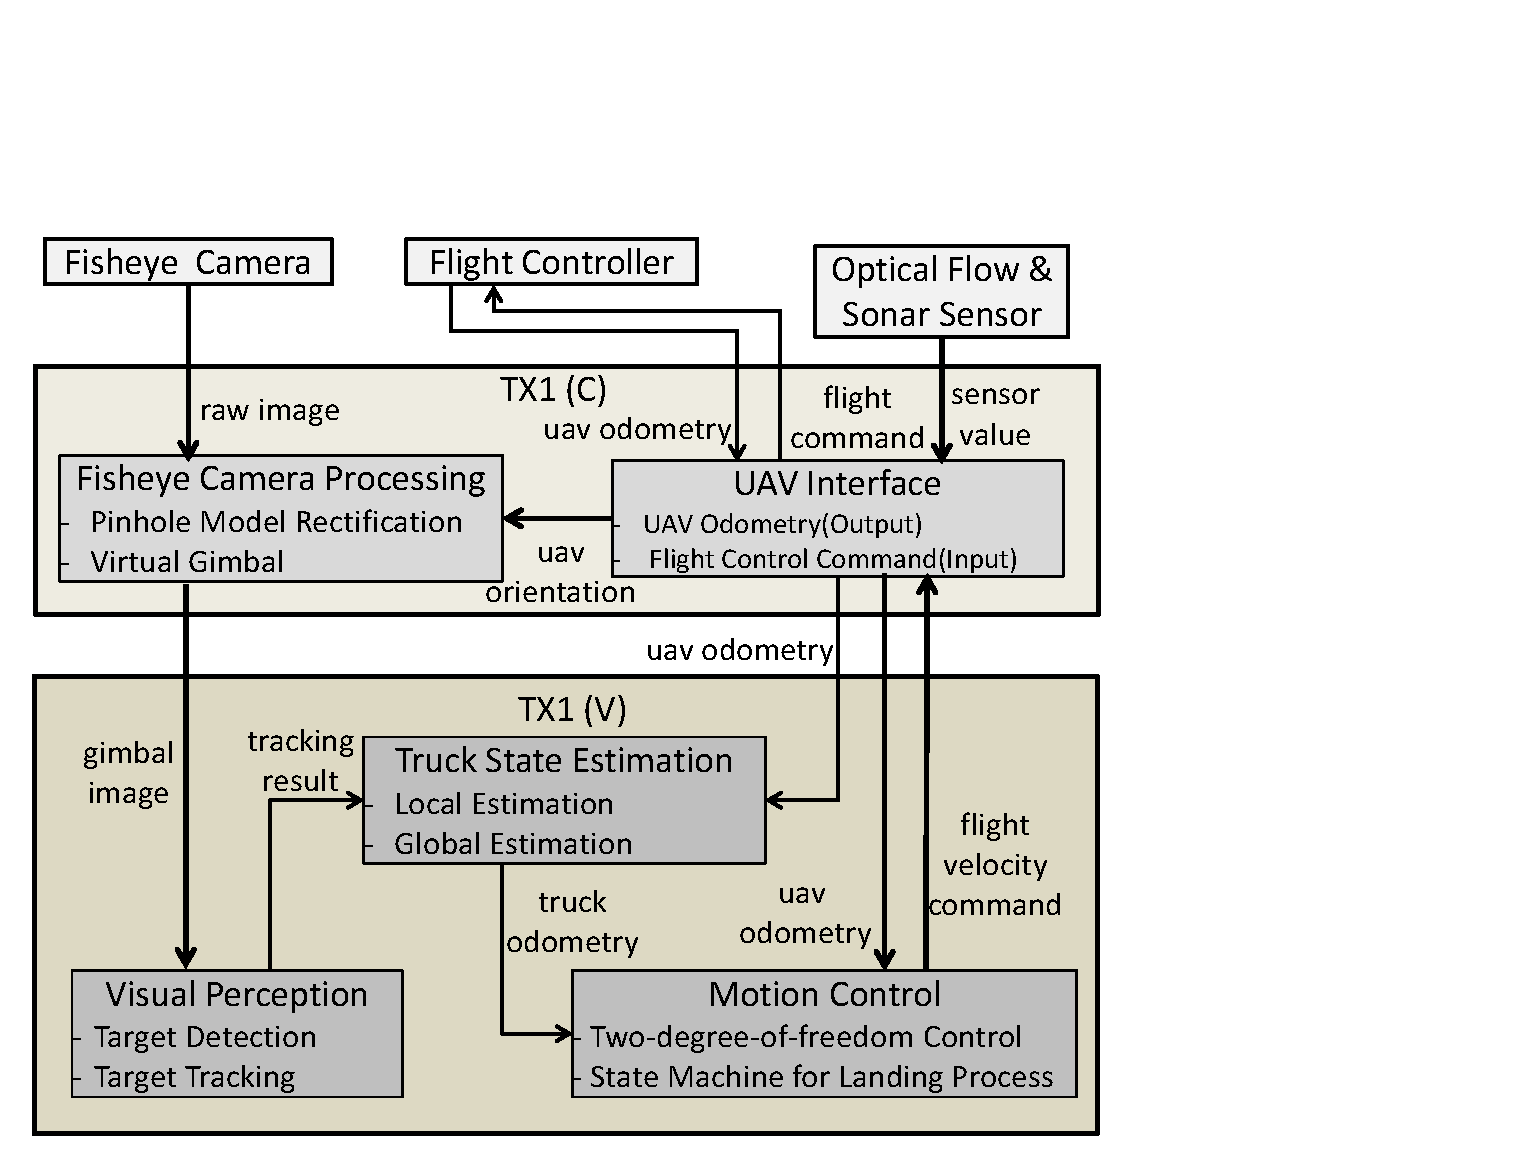
\includegraphics[clip, bb= 0 0 525 440, width=0.9\columnwidth]{sections/task1/images/task1_framework.eps}
          \end{center}
        \end{minipage}
    \end{center}
    \caption{Top: hardware platform DJI M100. Down: the system framework inside the platform.}
    \label{figure:task1-platform}
\end{figure}


\subsection{Software Environment}
The visual perception algorithms and motion control are implemented
on Robot Operating System (ROS) environment\footnote{\url{http://www.ros.org}}.
We used Gazebo\footnote{\url{gazebosim.org}} for virtual simulations
\footnote{\url{https://github.com/start-jsk/jsk_mbzirc}}. Our
algorithms are implemented in C/C++, Python and CUDA-C.


\subsubsection{Visual Perception}

The image processing is one of the fundamental component of autonomous
systems. With efficient and robust image processing the planning and
decision making can be done more readily which improves the accuracy
and robustness of executing the assigned task. Hence, one of our
primary objective while designing our software architectures was
real-time performance with minimal loss of accuracy. The visual
components of task one include three main stages described as follows:

\subsubsection{Fisheye Camera Processing}
To achive the image process based on the fisheye model, it is necessary to convert the raw image to pinhole model first. Besides, we also developed an original method called virual gimbal which combines the orientation data of UAV with the raw image data to calculate the level image frame Fig.\ref{figure:fisheye-virtual-gimbal}. This method is significantly important when the UAV tilts with large angle(e.g. $20^\circ$) while tracking the downward target.

\begin{figure}[h]
    \begin{center}
      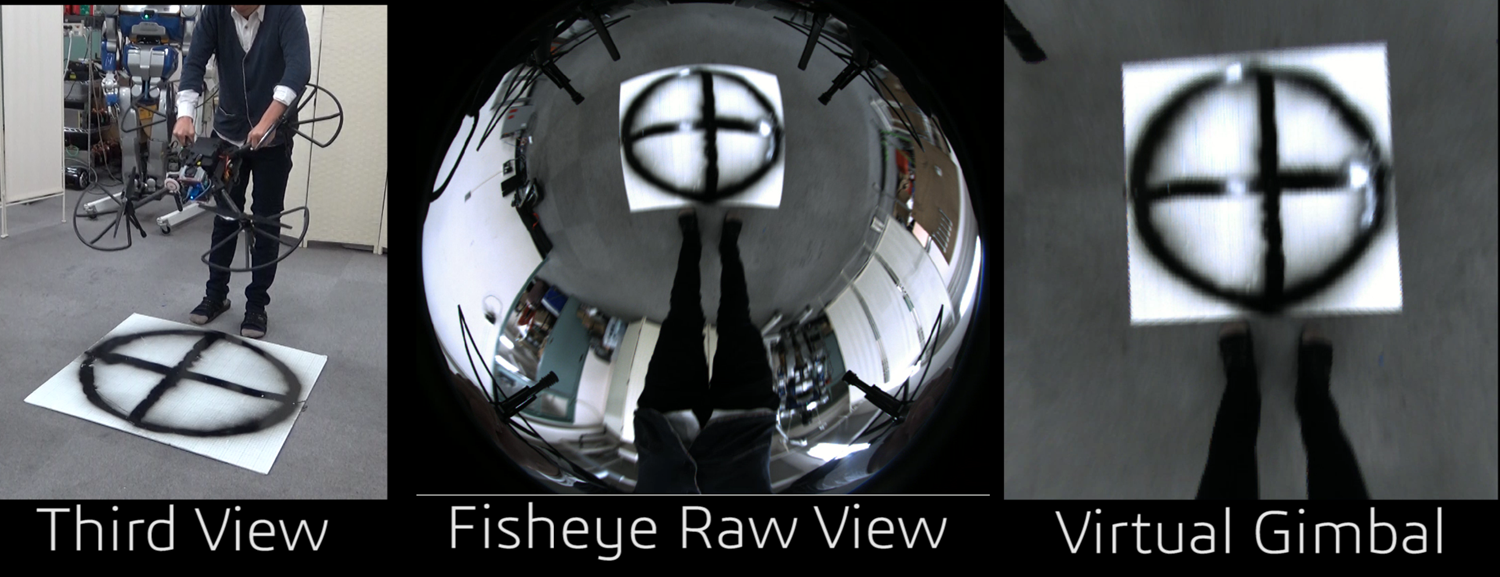
\includegraphics[width=0.9\columnwidth]{sections/task1/images/fisheye_virtual_gimbal.png}
    \end{center}
    \caption{Fisheye Virtual Gimbal}
    \label{figure:fisheye-virtual-gimbal}
\end{figure}

\subsubsection{Target Detection}
The target detection phase is the initial localization of the landing
region (heliport) on the truck. To detect the heliport we use the
traditional computer vision detection approach where by a sliding
window based method is used. However such raster scanning windows are
computationally expensive even for high end systems. To overcome this
crucial limitation we first generate candidate objectness
regions. Since the heliport is fixed to a moving target, we use
Gaussian based background subtractor fused with Kalman Filters for 
global motion compensation to generate regions of interest
(ROI)  with stable changes. The candidate ROI's are then ranked using
edge similarity between each sliding window. High scoring ROI are then
used for detecting the heliport using pretrained detector. 
Let $\mathbf{H}$ denote the detected target region.

\subsubsection{Target Tracking}

In order for an UAV to approach and land on the heliport online visual
feedback is very important given that the target is constantly moving.
Using the assumption that the target is not
expected to change abruptly both in terms of visual motion and
appearances, we use visual tracking for online feedback.
The detected region $\mathbf{H}$ is used to initialize the
tracker. Our visual tracking algorithm is highly efficient and robust
to both scale and visual changes and runs in real time, thus
providing frame by frame location of the target. To enable a tracker
to run online in real time we carefully crafted the expensive process
of feature computation by reducing it to one time process. 
The invariant features for tracking are computed by passing the image
through several pre-trained kernels of varying dimensions. By varying
the sizes of the kernel, an approximate scale can also be detected.
Moreover, the tracker is updated online at fixed intervals.

\begin{figure}[t!]
  \centering
  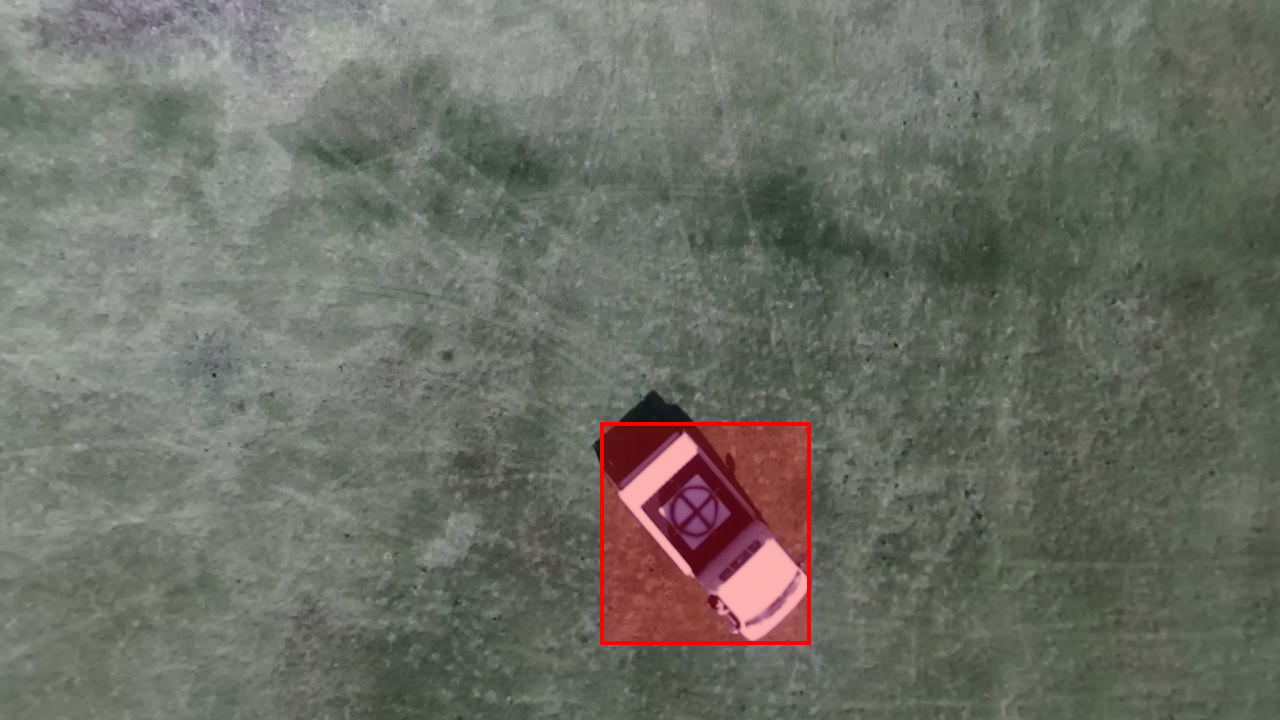
\includegraphics[height=1in]{sections/task1/images/detect2}
  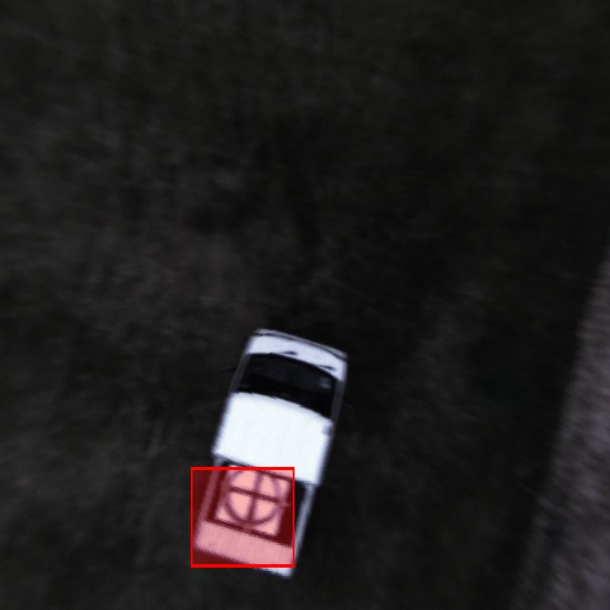
\includegraphics[height=1in]{sections/task1/images/detect1}
  \caption{Illustration of truck and heliport detection.}
\end{figure}

\subsection{Truck State Estimation}

{\bf TODO}

\subsection{Motion Control}

\subsubsection{Two-degree-of-freedom Control}
{\bf TODO}

\subsubsection{State Machine for Landing Landing Process}
{\bf TODO}

Our landing algorithm is closely cooperating with our robust tracking algorithm. We defined an inverted conical region related to the center of the tracking object. When UAV is stably moving in this region, UAV is considered tightly keeping in tracking with the moving object. Then UAV starts going down with stable speed. And our strategy is that when UAV is 0.3[m] higher than truck, we will stop going down and adjust to the most center of the parking apron and land directly and quickly to it. The reason is that currently our tracker in vision algorithm is to detect the inside circle region of parking apron, whose radius is 0.5[m], and the look-down fisheye camera we used is $120^\circ$  for perspective, so it means when UAV is 0.29[m] higher than parking apron, look-down camera could not cover the whole region. But 0.29[m] is already close enough for UAV to directly land, and our experiments also prove this strategy is practically feasible.


\subsection{Results Achieved to Date}

We have completed task one fully autonomously landing on the moving
target at 5[km/h], 10[km/h] and 15[km/h]. Moreover we demonstrate the effectiveness of our real time planning and tracking by showing the results of long time
following of the target at over 35[km/h]. The results of these tracking and landing motion are shown in video.

For landing control, we first test our method to land on fixed truck, and result shows that precision is below 10 centimeters, which is close to an start-of-the-work by HKUST's team in ICRA2015. And for moving object, we succeeded landing on truck with 15[km/h] as shown in Fig.\ref{figure:landing}.

\begin{figure}[h]
    \begin{center}
      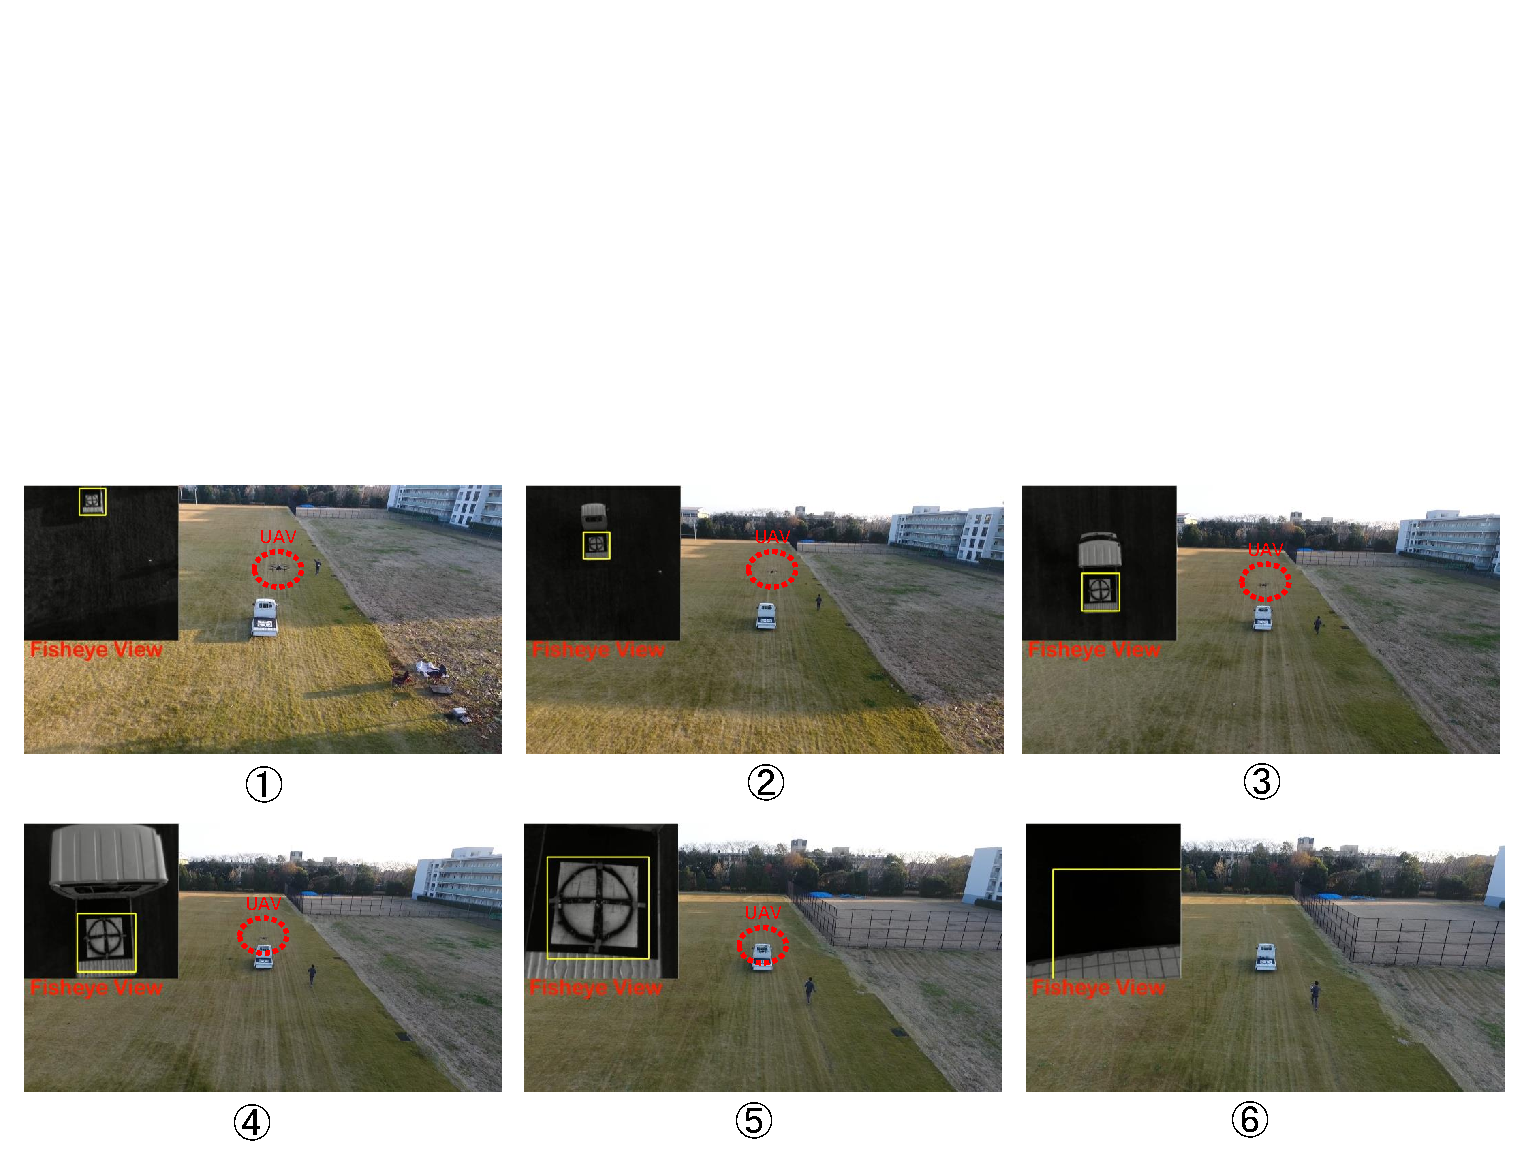
\includegraphics[clip, bb= 0 0 720 315, width=1.0\columnwidth]{sections/task1/images/task1_landing.eps}
    \end{center}
    \caption{The landing process in the case of [15Km/h]. For more details, please check our video.}
    \label{figure:landing}
\end{figure}


\subsection{Future Work}
\subsubsection{Landing Control}
Since outdoor landing when target object is moving in high speed is an unsolved difficult problem, currently our landing is also restricted in straight-road landing. However in the challenge, starting from center crosswords, only a 20[m] straight road is available. If considering truck is moving with 15 [Km/h] (~4 [m/s]), UAV has to land within 5[s]. Currently for development and safety consideration, our landing is slow and need around 15[s].
In next stage, we plan to reevaluate this academic problems and make pioneer trails to generate realtime landing trajectory for landing during target object is turning with high speed.


\end{document}
